\documentclass[a4paper, 11pt]{article}
\usepackage{lipsum} %This package just generates Lorem Ipsum filler text. 
\usepackage{fullpage} % changes the margin
\usepackage{mathpazo}
\usepackage{multicol}
\usepackage{graphicx, float}
\usepackage{enumerate}
\usepackage{pythonhighlight}
\usepackage{booktabs}
\usepackage{listings}
\usepackage[T1]{fontenc}
\usepackage[english]{babel}
\usepackage{amsmath,amsfonts,amsthm} % Math packages

\begin{document}
%Header-Make sure you update this information!!!!
\noindent
\large\textbf{Chapter 1} \hfill \textbf{Siyuan Feng (516030910575)} \\
\normalsize {\bf CS 391 Computer Networking} \hfill ACM Class, Zhiyuan College, SJTU\\
Prof.~{\bf Yanmin Zhu} \hfill Due Date: October 9, 2018\\
TA.~{\bf Haobing Liu} \hfill Submit Date: \today

\section*{P1}
	\subsection*{Request Format}
\hspace{14pt} All requests from client are in the same format
	\begin{lstlisting}
	REQUEST Bank Server Protocol/1.0
	CARD <card_number>
	PASSWORD <password>
	TRADE <trading_volume>
	END REQUEST
	\end{lstlisting}
	
There is no doubt about $card\_number$ and $password$. And here is some explanation about $trading\_volume$. $trading\_volume$ is change of the amount of money in the account after this request. That is if a user try to withdraw \$100, the $trading\_volume$ will be $-100$. On the contrary, if a user try to put in  \$50, the $trading\_volume$ will be $50$. When $trading\_volume=0$, this request will only query the balance in the account.
	
	\subsection*{Response Format}
	\begin{lstlisting}
	RESPONSE Bank Server Protocol/1.0
	CODE <return_code>
	MESSAGE <return_msg>
	END RESPONSE
	\end{lstlisting}
	
Here is a list for $return\_code$ and $return\_msg$ in different conditions.

	\begin{table*}[!htp]
		\centering
		\textbf{Table 1}~~Response Code and Message.\\
		\setlength{\tabcolsep}{7mm}
		\begin{tabular}{c c c} 
		\toprule
		return\_code & return\_msg & remark\\
		\midrule
		 0 & OK & no error\\
		1 & Login Failed & card number or password error\\
		2 & Withdraw Failed & do not have enough money\\
		3 & Unknown Errors & other error occupied \\
		\bottomrule
		\end{tabular}
	\end{table*}
	
\section*{P2}
\hspace{14pt} According to Equation 1.1, a single packet through $N$ links cost $N \frac{L}{R}$. The next packet send out after the first one in delay $\frac{L}{R}$, and the $P^{th}$ packet send out after $(P - 1)\frac{L}{R}$. Hence, the total delay will be $$d_{end\_to\_end} = (N + P - 1)\frac{L}{R}$$
	
\section*{P6}
	\begin{enumerate}[a.]
		\item $d_{prop} = m / s$
		\item $d_{trans} = L / R$
		\item $d_{end\_to\_end} = d_{prop} + d_{trans} = m / s + L / R$
		\item The last bit has just recent sent out from Host A.
		\item The first bit is on the way to Host B.
		\item The first bit has already received by Host B.
		\item According to the problem, $d_{prop} = d_{trans}$. That is $m / s = L / R $. Hence $$ m = s \frac{L}{R} = 5.36 \cdot 10^5 \text{meters}$$
	\end{enumerate}
	
\section*{P9}
	\begin{enumerate}[a.]
		\item $N_{circuit} = R / a = 10000$.
		\item The probability will be $$P(n > N) = \sum_{n=N+1}^M \begin{pmatrix} M \\ n\end{pmatrix} \cdot p^n \cdot (1-p)^{M-n}$$
	\end{enumerate}
	
\section*{P14}
	\begin{enumerate}[a.]
		\item $d_{total} = d_{queue} + d_{trans} = IL/R(1-I) + L/R = \frac{L}{R(1-I)} = \frac{L}{R - La}$
		\item According $I = La / R$. Let $x = L / R$, there is $d_{total} = \frac{x}{1 - ax}$. Here is plot.
		\begin{figure}[H]
			\centering
			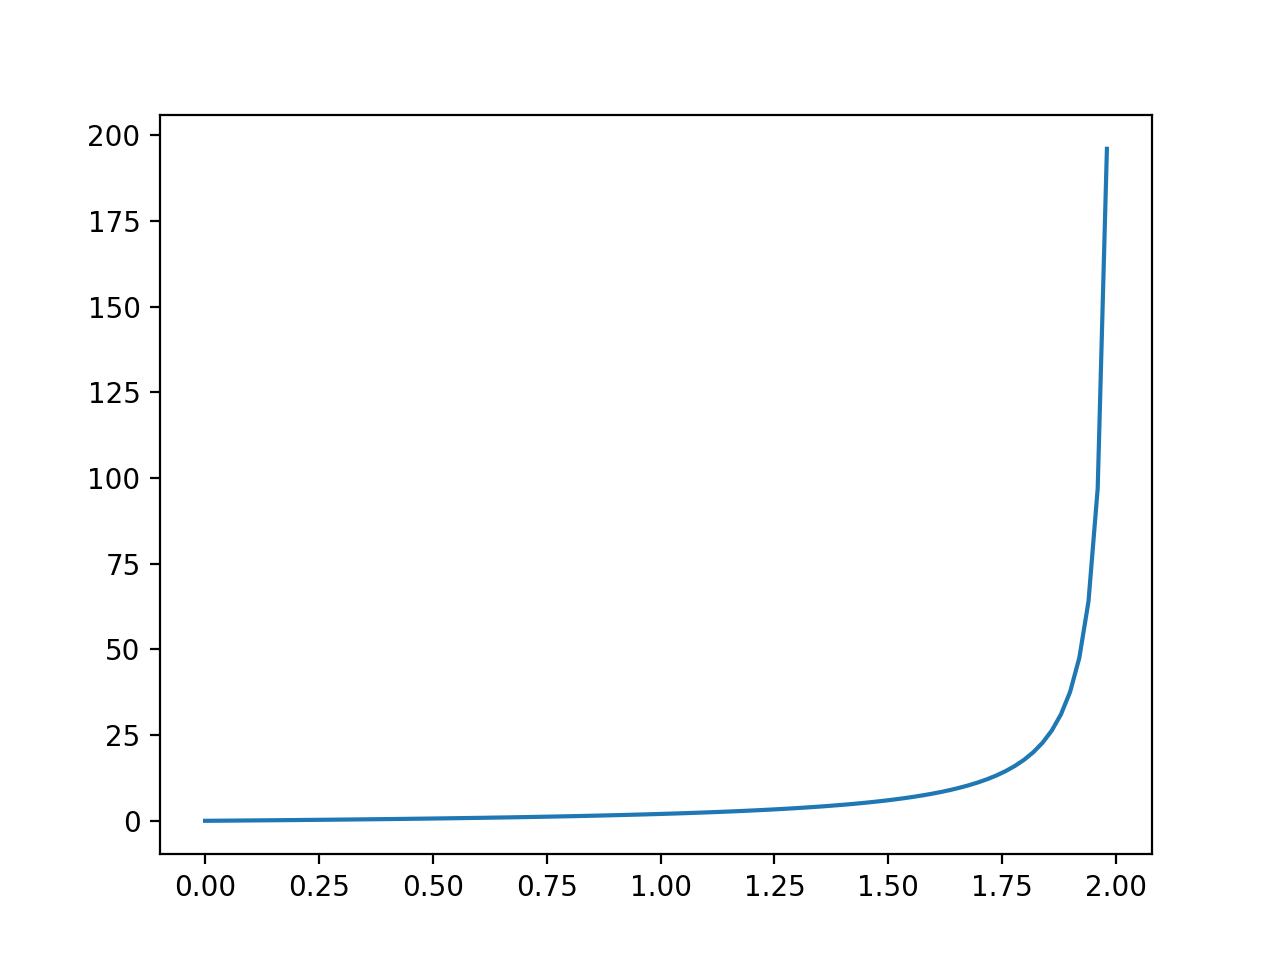
\includegraphics[width = 0.7 \linewidth] {Figure1}
			\caption{Delay function of $L / R$ with $a = 0.5$}
		\end{figure}
	\end{enumerate}
\section*{P16}
\hspace{14pt} The transmission delay $d_{trans} = 10 \text{ msec}$, and total delay $d = 20 \text{ msec}$. On average, there is only one packet is being transmitted. Then $N = 11$. 

According to Little's formula, $N = a \cdot d$. Hence, $$a = \frac{N}{d} = 550\text{ packets/sec}$$

\section*{P25}
	\begin{enumerate}[a.]
		\item The bandwidth-delay product $R \cdot d_{prop} = R \cdot m / s = 0.16\text{ Mb}$
		\item There are at most $0.16\text{ Mb}$ in this link at any given time no matter how large the file is. (In this case, the file must be larger than $0.16\text{ Mb}$)
		\item The bandwidth-delay product determines the maximum number of bits that will be in the link at any time.
		\item $Width_{bit} = m / (R \cdot d_{prop}) = s / R = 125 \text{meters}$, which is longer than a football field.
		\item $Width_{bit} = \min(m / (R \cdot d_{prop}), m) =  \min(m /(R \cdot m / s), m) = \min(s / R, m)$
	\end{enumerate}
\end{document}
